\documentclass[a4paper]{article}

\usepackage{pgfplots}
%\usepackage{tikz}

\usepgfplotslibrary{fillbetween}
\usepgfplotslibrary{patchplots}



\begin{document}


%\tracingmacros=2 \tracingcommands=2

% We use the polynomial f(x) -1/100 x^2 +2x .

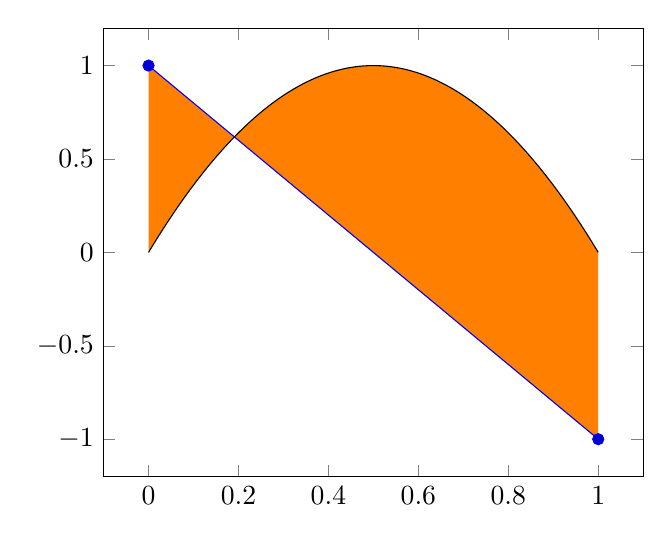
\begin{tikzpicture}
	\begin{axis}
	\draw[name path=A] (axis cs:0,0) .. controls (axis cs:0.333,1.3333) and (axis cs:0.66666,1.33333) .. (axis cs:1,0);
	
	%
	%\addplot+[name path=A,patch, point meta=none,patch type=quadratic spline]
	%	coordinates {(0,0) (1,0) (0.5,1)};
	
	\addplot+[name path=B] coordinates {(0,1) (1,-1)};

	\addplot[orange] fill between[of=A and B,reverse];
	\end{axis}
\end{tikzpicture}

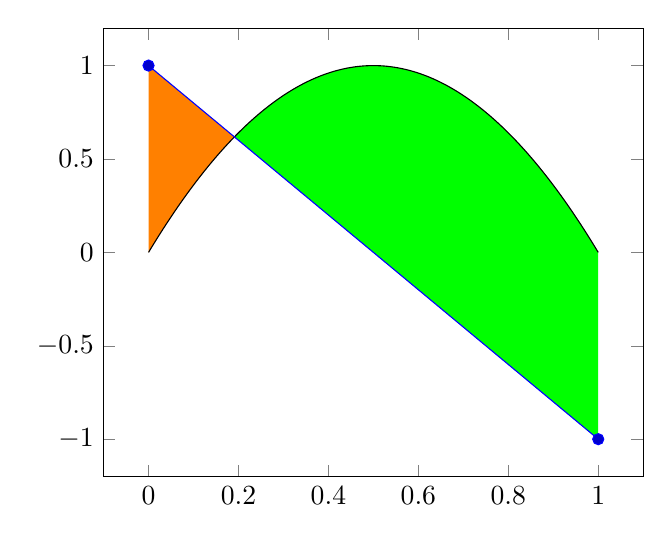
\begin{tikzpicture}
	%\tracingmacros=2 \tracingcommands=2
	\begin{axis}
	\draw[name path=A] (axis cs:0,0) .. controls (axis cs:0.333,1.3333) and (axis cs:0.66666,1.33333) .. (axis cs:1,0);
	
	\addplot+[name path=B] coordinates {(0,1) (1,-1)};

	\addplot[orange] fill between[%
		of=A and B,split,reverse,
		every odd segment/.style={green},
	];
	\end{axis}
\end{tikzpicture}

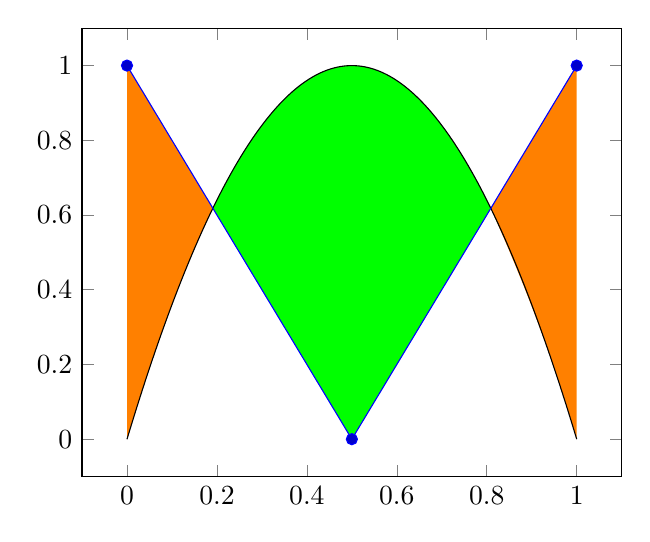
\begin{tikzpicture}
	%\tracingmacros=2 \tracingcommands=2
	\begin{axis}
	\draw[name path=A] (axis cs:0,0) .. controls (axis cs:0.333,1.3333) and (axis cs:0.66666,1.33333) .. (axis cs:1,0);
	
	\addplot+[name path=B] coordinates {(0,1) (0.5,0) (1,1)};

	\addplot[orange] fill between[%
		of=A and B,split,reverse,
		every odd segment/.style={green},
	];
	\end{axis}
\end{tikzpicture}

\iffalse
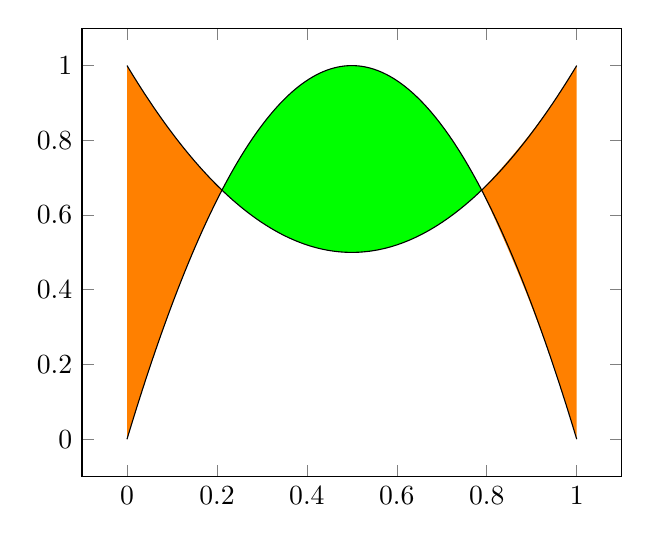
\begin{tikzpicture}
	\tracingmacros=2 \tracingcommands=2
	\begin{axis}[xmin=0,xmax=1,ymin=0,ymax=1,enlargelimits]
	\draw[name path=A] (axis cs:0,0) .. controls (axis cs:0.333,1.3333) and (axis cs:0.66666,1.33333) .. (axis cs:1,0);
	
	\draw[name path=B] (axis cs:0,1) .. controls (axis cs:0.333,0.3333) and (axis cs:0.66666,0.33333) .. (axis cs:1,1);

	\addplot[orange] fill between[%
		of=A and B,split,reverse,
		every odd segment/.style={green},
	];
	\end{axis}
\end{tikzpicture}
\fi
\end{document}


